\documentclass{beamer}
\usepackage[utf8]{inputenc}
\usepackage[brazil]{babel}
\usepackage{hyperref}
\usepackage{amssymb,amsmath}
\usepackage{subfigure}

\usetheme{Warsaw}
\bibliographystyle{abnt-alf}

\institute{Universidade Tuiuti do Paraná}
\author{Bogdano Arendartchuk}
\title{Avaliação de técnicas de predição de comportamento de máquinas
virtuais para a otimização de uso de parque computacional}
\date{\today}

\setbeamertemplate{footline}{
  \leavevmode%
  \hbox{%
  \begin{beamercolorbox}[wd=\paperwidth,ht=5.25ex,dp=1ex,right]{date in head/foot}%
    \insertframenumber{} \hspace*{2ex}
  \end{beamercolorbox}}%
  \vskip0pt%
}
\newcommand{\vect}[1]{\mathbf{#1}}
\newcommand{\norma}[1]{| #1 |}

\begin{document}

\frame{\titlepage}

\section{Contextualização}

\begin{frame}{}
\begin{block}{}
\centering
Avaliação de técnicas de predição de comportamento de \\
\textbf{{\color{red}máquinas virtuais}}
para a otimização de uso de parque computacional
\end{block}
\end{frame}

\begin{frame}
\begin{block}{Virtualização}
Consiste na execução simulada de cada instrução de uma determinada
arquitetura bem como a emulação de seu hardware original, de maneira a
permitir que qualquer sistema operacional compatível possa também executar
neste ambiente.\cite{goldberg1974survey}
\end{block}
\begin{itemize}
\item com auxílio de um \emph{software de virtualização}
\end{itemize}
\end{frame}

%% \begin{columns}[c]
%% \column{1.5in}
%% \center
%% \includegraphics[width=4cm]{dutra2009-arq-virtualizacao.png}
%% \column{1.5in}
%% Foo bar baz.
%% \end{columns}
\begin{frame}{Arquitetura clássica (ou típica)}
\begin{figure}
\centering
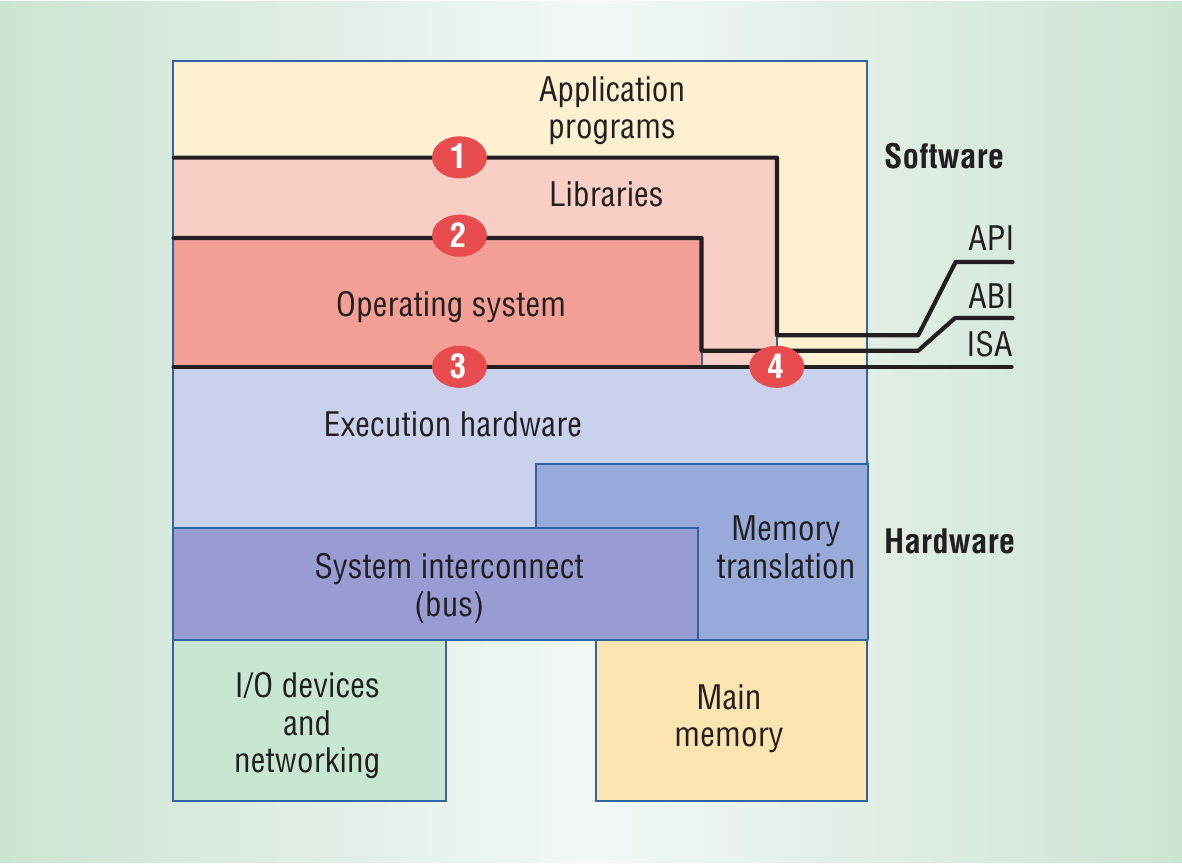
\includegraphics[height=5cm]{img/img-smith2005cla.png}
\end{figure}
\tiny{Fonte: \cite{smith2005architecture}}
\end{frame}

\begin{frame}{Arquitetura de virtualização}
\begin{figure}
\centering
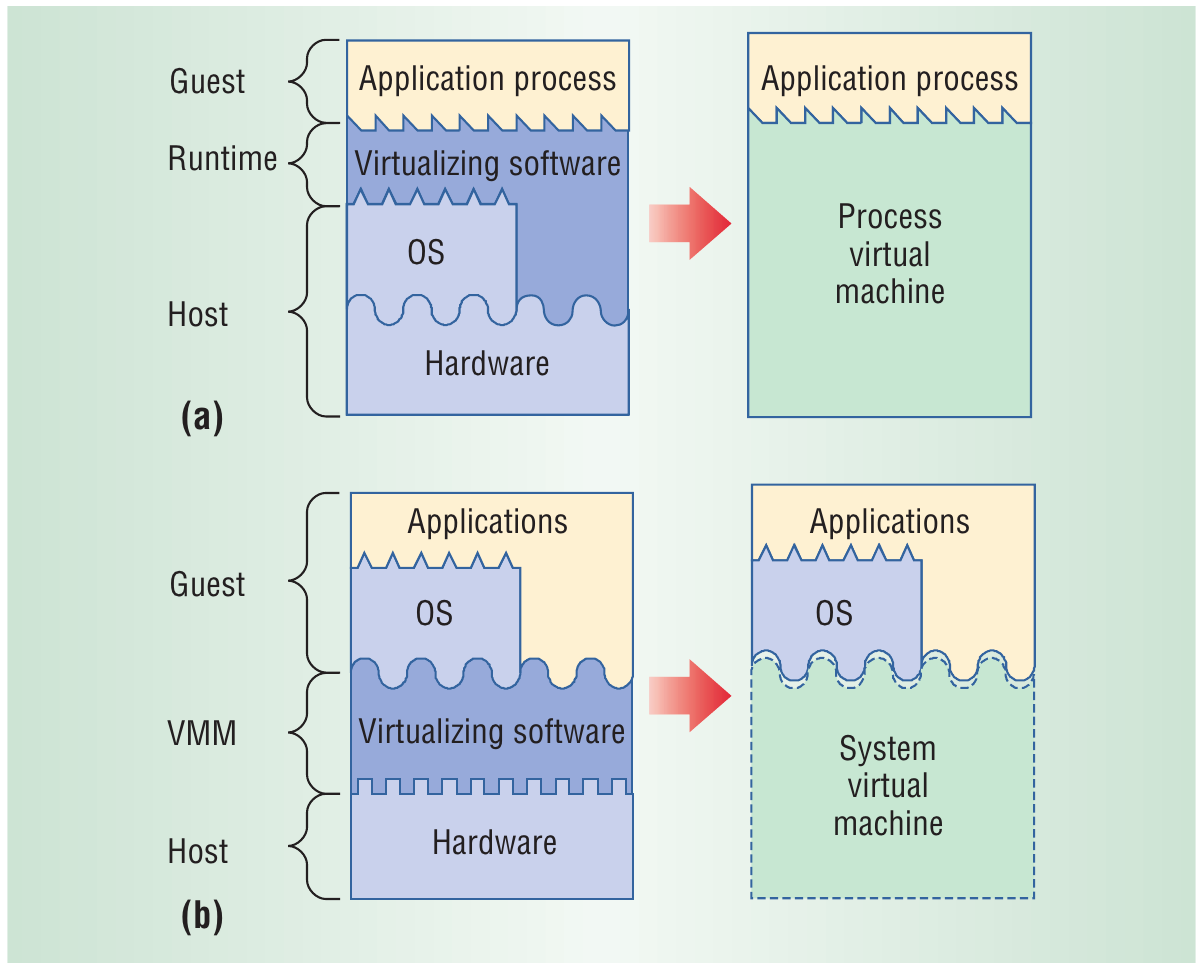
\includegraphics[height=5cm]{img/img-smith2005vir.png}
\end{figure}
\tiny{Fonte: \cite{smith2005architecture}}
\begin{itemize}
\item software de virtualização: \emph{monitor de máquinas virtuais}
\item máquina virtual: arquitetura + componentes de hardware simulados
\end{itemize}
\end{frame}

\begin{frame}{Monitores de Máquinas Virtuais}
% talvez citar que estão cada vez mais focados em cloud computing, blabla
\begin{columns}[c]
\column{1.5in}
\begin{itemize}
  \item VMware
  \item Xen
  \item Virtualbox
  \item QEMU
  \item KVM
\end{itemize}
\column{1.5in}
\begin{figure}
\centering
\includegraphics[height=3cm]{imgi-logos.pdf}
\end{figure}
\end{columns}
\end{frame}

%% \begin{frame}{\emph{libvirt}}
%% \begin{columns}[c]
%% \column{1.5in}
%% \begin{itemize}
%%   \item abstrai acesso aos MMV
%% \end{itemize}
%% \column{1.5in}
%% \includegraphics[height=2cm]{img-libvirt-contexto1.pdf}
%% \end{columns}
%% \end{frame}

\begin{frame}{Ambiente de virtualização I}
\begin{figure}
\centering
\includegraphics[height=5cm]{imgi-amb0.pdf}
\end{figure}
\end{frame}

\begin{frame}{Ambiente de virtualização II}
\begin{figure}
\includegraphics[height=5cm]{imgi-amb1.pdf}
\end{figure}
\end{frame}

\begin{frame}{Uso de processador}
\begin{figure}
\centering
\includegraphics[height=5cm]{imgi-amb-usocpu.pdf}
\end{figure}
\end{frame}

\begin{frame}{Migração}
\begin{figure}
\centering
\includegraphics[height=3.5cm]{imgi-amb-migracao.pdf}
\end{figure}
\end{frame}

\section{Metodologia}

\begin{frame}{Ferramenta objetivo}
\begin{figure}
\centering
\includegraphics[height=3.5cm]{imgi-amb-projeto.pdf}
\end{figure}
\end{frame}

\begin{frame}{Modelagem: componentes e interação}
\begin{figure}
\centering
\includegraphics[height=4.5cm]{img-met-contexto-1.pdf}
\end{figure}
\tiny{\url{http://libvirt.org}}
\end{frame}

\begin{frame}{Construção do vetor de características}
\begin{figure}
\centering
\includegraphics[height=4.5cm]{img-vetor-janela.pdf}
\end{figure}
\tiny{Como descrito e avaliado por \cite{frank2001time}.}
\end{frame}

\begin{frame}{Técnicas de aprendizado}
Técnicas avaliadas:
\begin{itemize}
\item $k$-Nearest Neighbours ($k$-NN),
\item \emph{Support Vector Machines} (SVM)
\end{itemize}
\end{frame}

\begin{frame}{\emph{Support Vector Machines} (SVM)}
\begin{itemize}
  \item publicado por Vapnik et al. (1995)\nocite{vapnik1998statistical}
  \item baseada no conceito de \emph{margem larga} (trata overfitting)
  \item figura!
  \item vetores de suporte são exemplos do conjunto de treinamento
  \item problema de otimiza\c{c}ão primal resolvido por meio de problema
dual
  \item aplicada com sucesso em: categorização de textos, reconhecimento de
voz e escrita à mão\cite{bennett2000support}
\end{itemize}

\begin{eqnarray}
& \label{eq:max_w0}\operatorname{Maximizar} & \frac{2}{\norma{\vect{w}}} \\
& \label{eq:max_w1} \operatorname{sujeito\;a} & y_i(\vect{w}\cdot\vect{x}_i + b) - 1 \ge 0 \quad i = 1,\dotsc,n.
\end{eqnarray}

\end{frame}

\begin{frame}{Support Vector Machines}
\begin{figure}
\centering
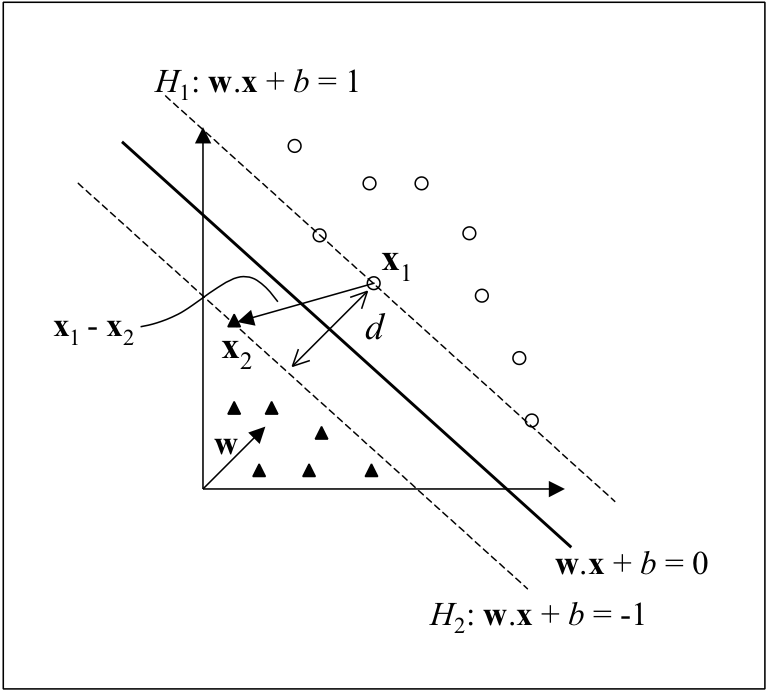
\includegraphics[height=5.5cm]{img/fig-hiperplanos.png}
\end{figure}
\tiny{Fonte: \cite{lorena2003introducaoas}.}
\end{frame}

\begin{frame}{Vetor de características para SVM}
\begin{figure}
\centering
\includegraphics[height=3cm]{img-vetor0.pdf}
\end{figure}
\begin{itemize}
\item valor contínuo é convertido em \textbf{categórico}
\item cada classe categórica resulta em uma SVM
\item classificação com várias SVMs: \emph{um-contra-todos}
\end{itemize}
\end{frame}

\begin{frame}{Testes}
Primera etapa:
\begin{itemize}
\item usos de CPU lidos de 5 máquinas a cada 30 segundos durante um mês,
\item este histórico será usado para avaliar o desempenho do previsor.
\end{itemize}
Então:
\begin{itemize}
\item com os melhores parâmetros para SVM e tamanho de janela, o histórico
será reproduzido em um conjunto de máquinas virtuais
\item reprodução do histórico será feita com \emph{busy loops}
\end{itemize}
\tiny{(Validação cruzada do histórico.)}
\end{frame}

\section{Resultados observados}

\begin{frame}{Dados coletados}
\begin{itemize}
  \item 80~200 valores lidos durante 27 dias
  \item ambiente: máquinas de compilação de software do projeto Mandriva Linux
\end{itemize}
\end{frame}

\begin{frame}{Valores coletados da máquina n4}
\begin{figure}
\centering
\includegraphics[height=5.5cm]{src/test-data/workload/dispersion-n4.png}
\end{figure}
\end{frame}

\begin{frame}{Histograma da máquina n4}
\begin{figure}
\centering
\includegraphics[height=5.5cm]{src/test-data/workload/histograma-n4.pdf}
\end{figure}
\end{frame}

\begin{frame}{Período de 4 horas da máquina n4}
\begin{figure}
\centering
\includegraphics[height=5.5cm]{src/test-data/workload/dispersion-4h-n4.png}
\end{figure}
\end{frame}

\begin{frame}{Busca de parâmetros}
\begin{figure}
\centering
\includegraphics[height=5.5cm]{src/test-data/classification/svm-n4-finer.pdf}
\end{figure}
\end{frame}

\begin{frame}{Desempenho de predição}
\begin{block}{Predição por hospedeiro}
\begin{table}
\centering
\begin{tabular}{| l | c | c | c | c | c | c |}
\hline
		& n2      & n3       & n4      	 & n6        & seggie  	 & média   \\
\hline
SVM     	& 99,32\%  & 99,78\% &   99,68\% &   99,34\% &   99,20\% & 99,46\% \\
\hline
$k$-NN  	& 97,22\%  & 99,04\% &   97,60\% &   96,88\% &   95,89\% & 97,33\% \\
\hline
\end{tabular}
\end{table}
\end{block}
\end{frame}

\begin{frame}{Testes de consolidação}
\begin{block}{Carga simulada de um dia}
\begin{table}
\centering
\begin{tabular}{| c | c | c | c | c | c |}
\hline
Técnica & Migrações & host0  & host1   & host2 & Dur. Simulação \\
\hline
$k$-NN 	& 98        & 24h    & 3:24:30 & 0h    & 12:31  \\
\hline
SVM 	& 120       & 24h    & 3:39:00 & 0h    & 02:23  \\
\hline
\end{tabular}
\end{table}
\end{block}
\end{frame}

\begin{frame}{Testes de consolidação}
\begin{block}{Carga simulada de uma semana}
\begin{table}
\begin{tabular}{| c | c | c | c | c | c |}
\hline
Técnica & Migrações & host0  & host1    & host2       & Dur. Simulação \\
\hline
$k$-NN 	& 510        & 168h  & 13:00    & 26:14:30    & 1:50:17  \\
\hline
SVM 	& 550        & 168h  & 13:30 	& 27:01:30    & 31:46  \\
\hline
\end{tabular}
\end{table}
\end{block}
\end{frame}

\begin{frame}{Hospedeiros utilizados}
\begin{figure}
\centering
\includegraphics[height=5.5cm]{src/test-data/scheduler/stats-svm-oneday-used.pdf}
\end{figure}
\end{frame}

\begin{frame}{Reprodução de carga real: uso de hospedeiros}
\begin{figure}
\centering
\includegraphics[height=5.5cm]{src/test-data/scheduler/stats-svm-real-oneday-used.pdf}
\end{figure}
\tiny{\emph{(Esperava-se o uso mais intenso dos três hospedeiros)}}
\end{frame}

\begin{frame}{Reprodução de carga real: demanda de CPU}
\begin{figure}
\centering
\includegraphics[height=5.5cm]{src/test-data/scheduler/stats-svm-real-oneday-tcc159.pdf}
\end{figure}
\tiny{\emph{(Demanda de CPU deveria exceder 400\%)}}
\end{frame}

\begin{frame}{Reprodução de carga real: comportamento esperado}
\begin{figure}
\centering
\includegraphics[height=5.5cm]{src/test-data/scheduler/stats-svm-oneday-host0.pdf}
\end{figure}
\tiny{\emph{(Demanda de CPU efetivamente excede o limite de 200\%)}}
\end{frame}

\begin{frame}{Reprodução de carga real: avaliando reprodução de carga}
\begin{figure}
\centering
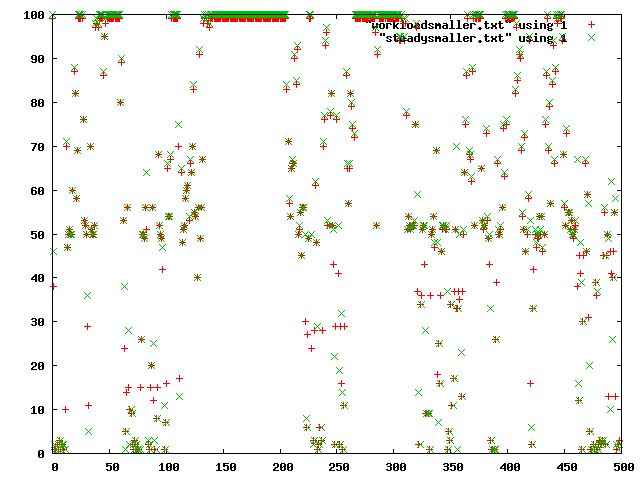
\includegraphics[height=5.5cm]{src/test-data/checking-load-simulator/load-simulator-n4.png}
\end{figure}
\tiny{\emph{(Carga aplicada em uma máq. virtual em um hospeiro)}}
\end{frame}

\section{Conclusões}

\begin{frame}{Conclusões}
\begin{itemize}
  \item foi possível antingir taxa de acerto de \emph{pelo menos} 97\% na
        predição de uso de CPU, para $k$-NN e SVM
  \item foi possível consolidar, de maneira simulada, a carga de 5 máquinas
        utilizando durante a maioria do tempo apenas dois hóspedes
  \item não foi possível reproduzir uma carga real em máquinas virtuais de
        maneira satisfatória para os testes
\end{itemize}
\end{frame}

\frame[allowframebreaks]{\frametitle{Referências}
  \bibliography{biblio}}
\frame{\frametitle{Dúvidas?} \centering{Dúvidas?}}

\end{document}
